\documentclass[12pt,reqno]{amsart}
\usepackage{amsthm,amsmath,amssymb}
\usepackage{mathtools}
\usepackage{proof}
\usepackage{subcaption}
\usepackage{centernot}
\usepackage{xcolor}
\usepackage{graphicx}
\usepackage[T1]{fontenc}
\usepackage{courier}
\usepackage{enumitem}
\usepackage{array}
\usepackage{multirow}
\usepackage{listings}
\lstset{basicstyle=\ttfamily\small, columns=fullflexible, language=sql}
\definecolor{mySucces}{RGB}{40, 167, 69}
\definecolor{myFail}{RGB}{220, 53, 69}

\newcommand{\code}[1]{\texttt{#1}}
\newcommand{\st}[0]{\text{ s.t. }}
\newcommand{\where}[0]{\text{ where }}
\newcommand{\pr}[0]{\text{Pr}}
\newcommand{\mand}[0]{\text{ and }}
\newcommand{\msgspc}[0]{\mathcal{M}}
\newcommand{\cphspc}[0]{\mathcal{C}}
\newcommand{\keyspc}[0]{\mathcal{K}}
\newcommand{\advrs}[0]{\mathcal{A}}
\newcommand{\oracle}[0]{\mathcal{O}}
\newcommand{\correctans}[0]{\colorbox{mySucces}{CORRECT}}
\newcommand{\falseans}[0]{\colorbox{myFail}{FALSE}}
\newcommand\MyBox[2]{
  \fbox{\lower0.75cm
    \vbox to 1.7cm{\vfil
      \hbox to 1.7cm{\hfil\parbox{1.4cm}{#1\\#2}\hfil}
      \vfil}%
  }%
}
\graphicspath{ {./} }
\newtheorem{theorem}{Theorem}[section]
\newtheorem{axiom}[theorem]{Axiom}
\newtheorem{case}[theorem]{Case}
\newtheorem{claim}[theorem]{Claim}
\newtheorem{conclusion}[theorem]{Conclusion}
\newtheorem{condition}[theorem]{Condition}
\newtheorem{conjecture}[theorem]{Conjecture}
\newtheorem{corollary}[theorem]{Corollary}
\newtheorem{criterion}[theorem]{Criterion}
\newtheorem{definition}[theorem]{Definition}
\newtheorem{example}[theorem]{Example}
\newtheorem{exercise}[theorem]{Exercise}
\newtheorem{lemma}[theorem]{Lemma}
\newtheorem{notation}[theorem]{Notation}
\newtheorem{problem}[theorem]{Problem}
\newtheorem{proposition}[theorem]{Proposition}
\newtheorem{remark}[theorem]{Remark}
\newtheorem{solution}[theorem]{Solution}
\newtheorem{summary}[theorem]{Summary}    
\begin{document}

\begin{center}
\large\textbf{Homework 4 \\ COMP530 Fall 2020 - Data Privacy and Security \\}
\normalsize\textbf{ Erhan Tezcan 0070881 \\ 10.01.2021} \\
\end{center}

\begin{center}
\line(1,0){250}
\end{center}

%
%\begin{enumerate}[label=(\alph*)]
%\item an apple
%\item a banana
%\item a carrot
%\item a durian
%\end{enumerate}
%

%	\begin{lstlisting}[language=sql]
%REVOKE ALL
%ON *
%FROM Frank
%	\end{lstlisting}

\section*{Answers}
\textbf{Answer 1:} 
\begin{enumerate}[label=(\alph*)]
\item This is a training-time attack. It is conducted during the retraining phases of the ML model.

\item The attack falls under the ``Integrity of the model'' category. It is making the model behave in unintended ways, and it adversarially modifies the model in doing so.

\item This is because Robinson's method (the method SpamBayes uses) assumes that the presence or absence of tokens in an email affect its spam status independently. The immediate implication of this is: if you add enough spam words in a valid mail, that mail will be scored as a spam eventually. That is why this attack works.

\item With the above observation, each words becomes a weapon on their own, and each word itself contributes to the spam score of a mail. So with this in mind, they first contaminate the model with valid words treated as spam, and actual valid mails that contain these words will as a result have higher spam score.

\item The idea is simple: our attack emails cause negative impact on the performance, thus if we reject mails that cause negative impact, it is likely that the rejected emails were attack emails.

\item The thresholds mentioned here are $\Phi_1$ and $\Phi_2$. These are used in the spam scoring: $[0, \Phi_0]$ means \textit{ham}, $(\Phi_0, \Phi_1]$ means \textit{unsure} and $(\Phi_1, 1]$ means \textit{spam}. Normally, these are determined by the user, or some default value. With the dynamic threshold defense, these thresholds values are shifted. The idea behind this comes from an observation: the attacks mentioned in the paper increase the spam score of both ham and spam mails. So by shifting the thresholds, we can expect to defend against such attacks.

\item In section 5.1, they mention that for the dictionary attacks, an attack message causes at least an average decrease of 6.8 has-as-ham messages. Whereas, non-attack spam messages cause at most an average decrease of 4.4 ham-as-ham messages. So there is a very clear line between these two. In particular, the attack message average decrease may be an outlier, compared to non-attack messages. By doing outlier analysis on this metric, we may be able to defend against dictionary attacks.
\end{enumerate}

\textbf{Answer 2:} 
\begin{enumerate}[label=(\alph*)]
\item Transferability is done in a black-box attack, where the adversary only has an oracle access to obtain labels on a data, but nothing else (especially regarding the internal architecture of ML model).

The idea is: ``samples crafted to mislead a model A are likely to mislead a model B''. Notice how if A is white-box but B is black-box, I can still mislead the black-box model, which mallicious data I had crafted for A. This is called the \textbf{transferability} property of adversarial examples.

\item In cross training data transferability, you partition your training data, and for each of them you craft adversarial examples, and see how misleading they are on the same type of model that were trained on other partitions of the data. It turns out that indeed, the misleading can be observed.

In cross technique transferability, you craft adversarial examples with some model and data, and see how misleading they are on other types of models trained on the same data.

So the major difference is: in cross training data transferability you are working with the same type of model, for example both the source and target models are same type (DNN, DT, SVM etc.), however in cross technique data your source and target models can be different. In particular, you could have an ensemble of models as target, where the ensemble looks at a majority vote during decision making.

\item They query the online blackbox ML model and with their responses, they generate synthetic data on their local model. Once the local model reaches a certain accuracy, they can use these synthetic data to actually craft adversarial examples to mislead the online model. Basically, the lack of training data is solved by synthetic data generation, and the lack of model is solved by transferability.

\item It does help to some extent, but still it is not as robust as single models such as Deep Neural Networks or k-Nearest Neighbor. He shows the results of percentage of misclassified data, in particular at around minute 11. 

\item Better understanding adversarial examples help us trust our ML model. For example, we can gain more trust on how an autonomous driving car can behave on unexpected and untrained data in the real world. Another example is that, on a ML model trained to tell us how well drugs perform for some disease, we can backpropagate it to perhaps create a synthetic drug that works better than all of them. However, this drug may actually be adversarial: it performs good on the model but is actually unhealthy. Understading and defending against adversarial examples will help us overcome these problems.
\end{enumerate}


\textbf{Answer 3:}
\begin{enumerate}[label=(\alph*)]
\item This is a test-time attack. It is conducted on an already trained model.

\item The attack falls under ``Integrity of the Model'' category. Notice that there is no access to training data, and it is a white-box attack as in they have access to the ML model and the test data. Furthermore, they want to create new adversarial examples as test data, to mislead the ML model. 

\item Consider an input $x$. An untargeted adversarial example is an input $x'$ such that $x$ and $x'$ are ``hard to distinguish from one another'' but the ML model assigns them different labels. In the targeted case, again we have such $x'$, but now we want the ML model to assign $x'$ to a label of our choice, i.e a target label. For example, consider an audio sounds like: \textit{firetruck} and the correct label is indeed \textit{firetruck}. An untargeted adversarial example would be an audio that sounds like \textit{firetruck} again, but perhaps labeled as \textit{fired rock}. A targeted adversarial example could have any label, say \textit{cheeseburger} but still somehow sound like \textit{firetruck}.

\item They measure the amount of perturbation in audio adversarial examples using Decibels. More formally, when an audio $x$ is perturbed with $\delta$, they measure the perturbation as $dB(\delta)-dB(x)$ where $dB$ measure the decibels of the audio. The perturbation is hard to notice by human ear, if this measured decibels are low, which means it is quiet.

\item In seciton 3-B, they basically use a linear programming method, where they try to obtain a perturbed audio with the minimum perturbation, but is classified with a target label by the ML model. In section 3-C they further improve their loss function, especially with regards to the audio domain, as many prior work seems to be on image domain. To hide speech, they give the target label as a sequence of space characters.

\item \begin{itemize}
	\item \textbf{Adversarial Training}: The ML model can be trained with some adversarial examples. Given the fact that these are all generated optimally, I think this may work to some extent. However, what if the adversary generates new audio from the tests of this more robust ML model? I think there is still a little bit of room for attack here.
	\item \textbf{Denoising}: I am not sure how well this would work against the attack, given the very low decibels of the perturbation, however if it can perhaps nullify the perturbations then it could prevent attacks. But I am pretty sure the attack will not be prevented by this one, the perturbations are very very small.
	\item \textbf{Ensemble Learning}: Several different ML models can be trained, that have several similar audio inputs that map to same target. The adversarial example will be crafted from a single test instace, and though it my fool the ML model that trained on the particular instance, other ML models can detect the problem, and given enough ML models the majority vote can recover from the attack.
			
\end{itemize}

\end{enumerate}

\newpage
\textbf{Answer 4:} 

\textit{In all of the answers below, the results are taken average over 25 iterations for each question. The program also prints pretty outputs to the console, if you would like to run.}

\begin{enumerate}[label=(\alph*)]
\item In figure 1, we see how accuracy is affected by label flipping and clean-label flipping attacks. 
\begin{figure}[ht]
 	\label{fig:lblflip}
 	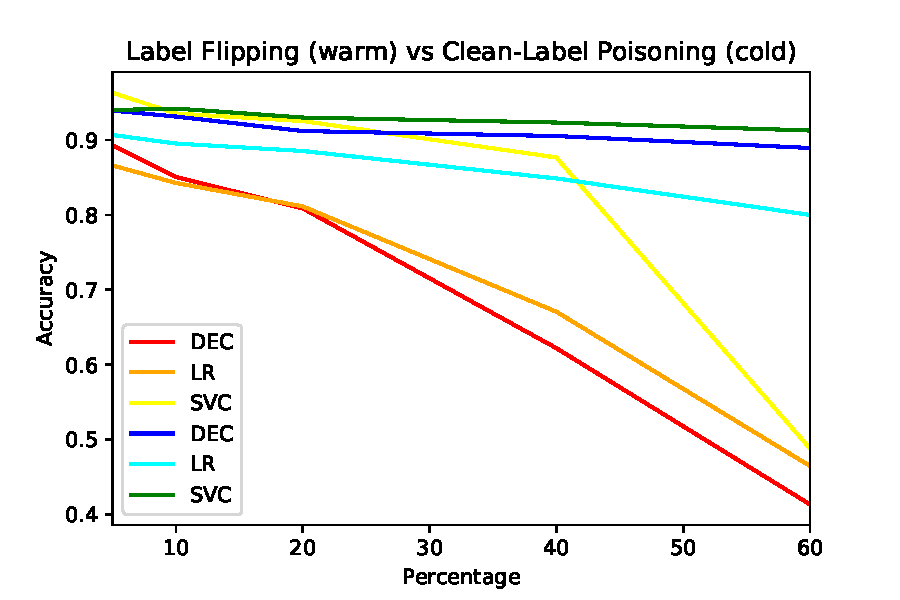
\includegraphics[width=0.8\linewidth]{labelflip.pdf}
 	\caption{Percentage and Accuracy for label flipping attacks (red, orange, yellow) and clean-label poisoning (blue, cyan, green).}
\end{figure}
Looking at this figure, we see that label flipping is definitely detrimental to the accuracy. SVC model seems to be more resilient to this attack, but still after around 40 percent of labels flipped we start to see a sharp decline. In general, we can say that label flipping attack succeeds to drop the accuracy in all of these models. We will explain the clean-label poisoning attack on the next bullet.

\item For our attack, we treat the machine learning algorithm like a query $\advrs : X \to Y$. Here, $X$ is the dataset and $Y$ is the label set. $\advrs (x \in X) = y \in Y$ somehow returns you the label of $x$. In our approach, we assumed that this query basically picks a random label for $x$ by looking at the dataset at hand. Let $|X_y|$ show the number of elements in $X$ that have label $y \in Y$.
$$
\Pr[\advrs(x) = y] = \frac{|X_y|}{|X|}
$$
One thing to note here is that we are querying an instance in data, rather than the dataset itself. This is wrong, but this method will still serve our purpose. We can naively treat the data instance as a dataset with 1 record, and look at the dataset information as common knowledge, given the fact that this attack is in a white-box setting. 

When a new element is added, it has probability $1/|Y|$ of belonging to same label. Call this new element $x^*$,
$$
\Pr[\advrs(x^*) = y] = \frac{1}{|Y|}\frac{|X_y|+1}{|X|+1} + \frac{|Y|-1}{|Y|}\frac{|X_y|}{|X|+1}
$$
From this, we get:
$$
\Pr[\advrs(x^*) = y] = \frac{|X_y||Y|+1}{|X||Y|+|Y|}
$$
Recalling the inequality for $\epsilon$-DP:
$$
\frac{\Pr[\advrs(x^*) = y]}{\Pr[\advrs(x) = y]} \leq e^{\epsilon}
$$
We look at:
$$
\frac{\Pr[\advrs(x^*) = y]}{\Pr[\advrs(x) = y]} = \frac{|X_y||Y|+1}{|X||Y|+|Y|}\frac{|X|}{|X_y|}
$$
$$
\frac{\Pr[\advrs(x^*) = y]}{\Pr[\advrs(x) = y]} = \frac{|X||X_y||Y|+|X|}{|X||X_y||Y|+|X_y||Y|}
$$
Notice here how if there were equally many data points of all labels, we would have $|X|/|Y| = |X_y|$ and thus $|X| = |X_y||Y|$ which would make the expression above to be 1. That would emply $\epsilon=0$. However, that is hard to bump into in real world, so we can process to find the $\epsilon$ by:
$$
\epsilon = \underset{y \in Y}{\max}\left(ln\left(\frac{\Pr[\advrs(x^*) = y]}{\Pr[\advrs(x) = y]}\right)\right)
$$
$$
\epsilon = \underset{y \in Y}{\max}\left(ln\left(\frac{|X||X_y||Y|+|X|}{|X||X_y||Y|+|X_y||Y|}\right)\right)
$$
As for the sensitivity, we have found that removing a data point with label $y$ affects the query most when the queried $x$ has label $y$, which gives:
$$
s = \frac{|X_y|}{|X|} - \frac{|X_y|-1}{|X|-1} = \frac{|X|-|X_y|}{|X|(|X| - 1)} 
$$

With these in mind, to all features $f$ in our data, we add laplace noise $lap(0, s/\epsilon)$. We then round the values to 1 decimal places, because that is how the data we had was. So, by looking it should not possible to notice the difference! One last thing, there may be some negative values sometimes, so to counteract that we also take the absolute value. In short, we map every feature $f$ to:
$$
|\lfloor f + lap(0, s/\epsilon) \rceil|
$$
where $\lfloor x \rceil$ rounds $x$ to nearest value to 1 decimal places. After some experiments, I decided to actually relax the sensitivity a little bit, I am actually using $0.1$ of the sensitivity in the code. I have observed that it is harder to distinguish that from the true dataset. So finally what we do is:
$$
|\lfloor f + lap(0, 0.1\times s/\epsilon) \rceil|
$$
Looking again at figure 1, we see how the accuracy is affected by the clean-label poisoning attack. Our attack is not too effective against DEC and SVC, though still we see a drop of around 0.5 accuracy on both of them. For LR however, we see a sharper drop, almost from 0.9 to 0.8. Keep in mind that our attack is performed in such a way that, it is very hard to distinguish instances of it from the normal training data. In fact, when we do clean-label poisoning over the whole training dataset, the average L1 norm of the difference between poisoned and true data turns out to be around 1.5. If you would like, please run the code and in a variable explorer try to distinguish the poisoned data from the training data! 

\begin{figure}
\centering
\begin{subfigure}{.5\textwidth}
  \centering
  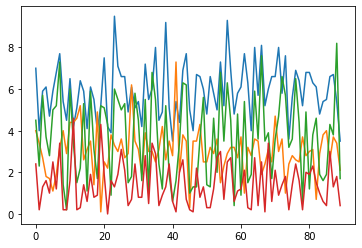
\includegraphics[width=.8\linewidth]{cleanlabel.png}
  \caption{100\% poisoned training data.}
  \label{fig:sub1}
\end{subfigure}%
\begin{subfigure}{.5\textwidth}
  \centering
  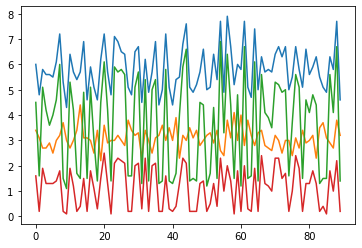
\includegraphics[width=.8\linewidth]{train.png}
  \caption{True training data.}
  \label{fig:sub2}
\end{subfigure}
\caption{Only when we look at the hundred percent poisoning we can notice the poison, which reflects as a form of noise, i.e. the figure seems sharper. However, when a smaller percentage of data is poisoned, this will be impossible to distinguish from the natural sharpness of the true data. Indeed, the accuracy is not affected too much, but it drops nevertheless.}
\label{fig:test}
\end{figure}

\item  We do our backdoor attack as follows: we first take the average of all features for data with the same label. Without loss of generality, call this label $y$. For every feature $f$, we take the average of that feature over all data with label $y$. After doing this to every feature, we have an average sample that is expected to correspond to that label. Note that this is a bit naive approach, and disrespects the topology (a similar problem to K-means not working when data is spatially classifiable but they share the same center). However, for this dataset we thought it may work. After obtaining the average data instance, we choose a feature and set it's value to our trigger. In our examples, we set the first feature to be 999. 
\begin{figure}[ht!]
 	\label{fig:backdoor}
 	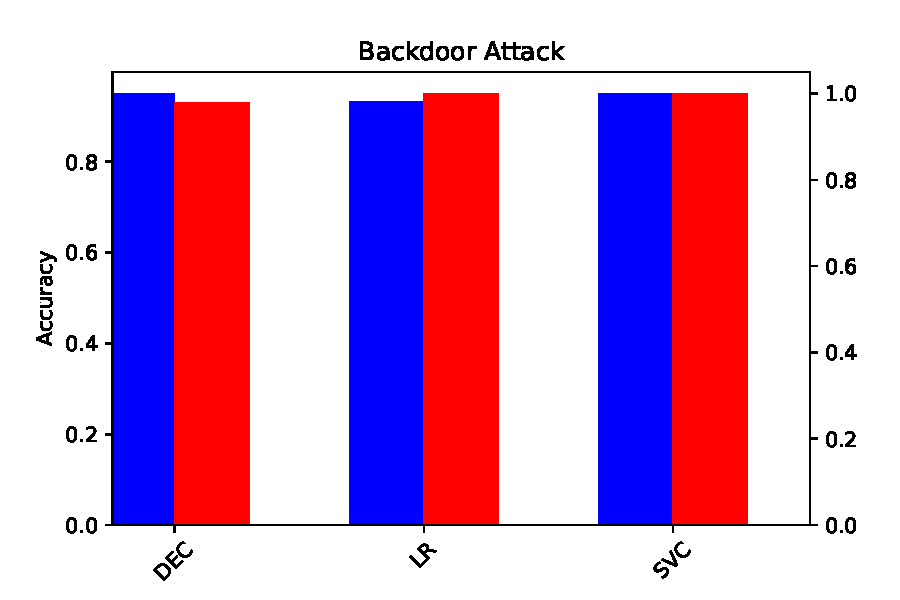
\includegraphics[width=0.8\linewidth]{backdoor.pdf}
 	\caption{Backdoor Attack. Blue bar shows the performance against existing test data. Red bar shows the performance against our adversarial examples.}
\end{figure}
In our attack, we only add \textbf{3 backdoored instances to the training data}, one for each label. Looking at figure 3, we see that the overall accuracy of backdoor-trained models against existing test data is not affected, in fact it is close to 95\% on all models. To test how well our trigger works, we create 10 instances of test data by sampling the existing dataset and adding our triggers to it. As seen in the red bar in figure 3, it is almost always misleading the model, i.e. our trigger caused the model to return the label we wanted. In LR and SVC we have 100\% accuracy, but in DEC we have 98\%. Note that sometimes, we get 100\% on all of them.

\item In this attack setting, we treated the problem as a black-box attack. Furthermore, we created our evasion instance just by working with DEC model, so that ensemble model may have more chance at resisting. To evade the model, we iteratively add a small laplace noise ($laplace(0, 0.01)$) to features of the test instance. In each iteration, the feature to add noise is chosen randomly, and we always check if the label is changed or not. After every 1000 iterations, the scale parameter of laplace noise is increased from its current $s$ to $1.1s$. We measure our perturbation by looking at the L1 Norm of the difference between original data and perturbed data, and the average turns out to be  around 1. This value sometimes goes to 1.5, or sometimes even as low as 0.5.

\item We look at a test data of 10 adversarial examples. The ensemble model has around 60\% accuracy on classifying our adversarial examples to their correct labels. So, it is not that effective, compared to 95\% accuracy of the normal models against true data.

\end{enumerate}






\end{document}